% This is the project description we were provided we can tailor it later

Silicate glasses are used widely, in fields that include medicine, optics, electronics, telecommunication and energy. While these materials have numerous benefits in terms of strength and resilience, they are also brittle. When placed under sufficient tensile stress, glasses fracture rather than stretch. The fractures grow, propagating through the glass and ultimately leading to material failure. In spite of considerable study, the nanoscale origins of fracture and the relation of atomic structure to fracture nucleation remain poorly understood.

A natural hypothesis might be that fracture nucleation is related to the presence of atomic-scale defects or chemical bond weakness in the glass. However, the relationship between atomic structure and fracture behavior is complex. Fractures do not simply originate at the site of the weakest link or most easily broken bond, and trigger further fracturing in the surrounding bonds~\cite{markpres}. Similarly, glasses with an increased density of nanoscale voids and defects do not necessarily display increased brittle behavior, and can even be better at absorbing stresses from mechanical deformation~\cite{pedone2015dynamics}. Instead, the nucleation and propagation of fractures appear to depend on more subtle characteristics of the local structure surrounding an atom.

\subsection{Physical Structure}

The basic molecular unit in a silicate glass is a silicon (Si) atom bonded to four oxygen (O) atoms in a tetrahedral configuration.  Each of these SiO$_4$ units can share its O atoms with neighboring tetrahedra.  An O atom shared between two molecules in this way is known as a \emph{bridging oxygen}, as seen in Figure~\ref{fig:tetrahedra}.

\begin{figure}[!b]
    \centering
    \noindent
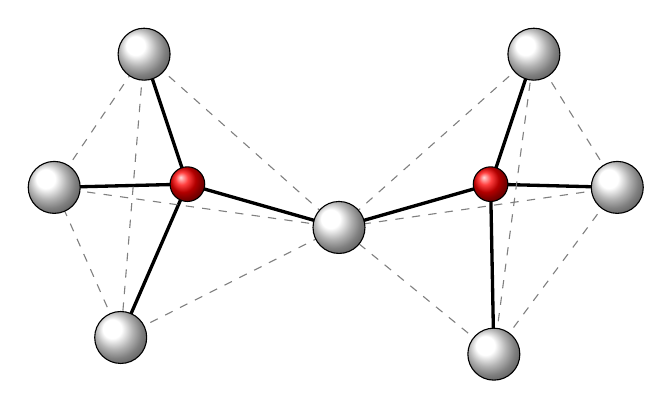
\begin{tikzpicture}[scale=1.1]
\coordinate (A) at (-0.5,0.5,0); % Left back O 
\coordinate (B) at (2,0.5,4.5); % Left front O  
\coordinate (C) at (6,0.5,0); % Right back O
\coordinate (D) at (6.5,0.5,5); % Right front O 
\coordinate (E) at (3.75,1,2.5); % Bridging Oxygen 
\coordinate (F) at (5.5,1.5,2.5); % Right Si
\coordinate (G) at (2,1.5,2.5); % Left Si 
\coordinate (H) at (1.5,3,2.5); % Left top O 
\coordinate (I) at (6,3,2.5); % Right Top O

%connections from left Si
\draw [very thick] (G) -- (A);
\draw [very thick] (G) -- (B);
\draw [very thick] (G) -- (H);
\draw [very thick] (G) -- (E);

%connections from Right Si 
\draw [very thick] (F) -- (C);
\draw [very thick] (F) -- (D);
\draw [very thick] (F) -- (I);
\draw [very thick] (F) -- (E);

%dashed lines between Oxygen. This can be removed but it was in literature. 
\draw[gray,dashed] (A) -- (H);
\draw[gray,dashed] (H) -- (B);
\draw[gray,dashed] (B) -- (A);
\draw[gray,dashed] (A) -- (E);
\draw[gray,dashed] (H) -- (E);
\draw[gray,dashed] (B) -- (E);

\draw[gray,dashed] (I) -- (C);
\draw[gray,dashed] (C) -- (D);
\draw[gray,dashed] (D) -- (I);
\draw[gray,dashed] (I) -- (E);
\draw[gray,dashed] (D) -- (E);                                                
\draw[gray,dashed] (C) -- (E);                                                


%place non-atom cube corners
\shadedraw [ball color= white] (A) circle (0.3cm);
\shadedraw [ball color= white] (B) circle (0.3cm);
\shadedraw [ball color= white] (C) circle (0.3cm);
\shadedraw [ball color= white] (D) circle (0.3cm);
\shadedraw [ball color= white] (E) circle (0.3cm);
\shadedraw [ball color= red] (F) circle (0.20cm);
\shadedraw [ball color= red] (G) circle (0.20cm);
\shadedraw [ball color= white] (H) circle (0.3cm);
\shadedraw [ball color= white] (I) circle (0.3cm);
\end{tikzpicture}
    \caption{Two silicon atoms (small red balls) with surrounding oxygen atoms (large grey balls) in tetrahedral configuration.  One bridging oxygen is at a corner shared by the two tetrahedra.}
    \label{fig:tetrahedra}
\end{figure}

When an Si atom is surrounded by $n$ bridging O atoms, it is called a Q$_n$ unit~\cite{shelby2005}. In a network of Q$_4$ units, all O atoms are shared between two Si atoms, forming a silicon dioxide (SiO$_2$) structure.  The network geometry can be regular, in which case the material is a crystal such as quartz.  Alternatively, the geometry can be irregular, in which case it is a glass.  When the network has Q$_n$ units with $n<4$, some of the O atoms surrounding an Si atom are non-bridging.

An Si atom can also be undercoordinated, bonding with fewer than four O atoms, or overcoordinated, breaking the tetrahedral symmetry and bonding with more than four O atoms.  In the latter case, this can result in rare Q$_n$ units with $n>4$~\cite{pedone2015dynamics}.

% Typically in these silicate glasses there exists a structure where silicon (Si) is surrounded by four oxygen (O) atoms forming a tetrahedron seen in Figure 1. These tetrahedra share one common O atom if they are neighbors. A ring forms if a group of tetrahedra share common O atoms, and the size of these rings is computed based on how many Si atoms are in the ring. A large ring has 11 and 12 Si atoms, medium rings have 5 and 6, and small rings have 1 or 2. An atom is denoted as under-coordinated if the number of its constraints is lower than 4, and over-constrained, if greater than 4. \cite{pedone2015dynamics}
% \begin{figure}
%     \centering
%     \noindent
%     \includegraphics[width=12cm, height=6cm]{picture/tetra.JPG}
%     \caption{Example of a primitive sixfold ring (left), example of a primitive twelve-fold ring
% (right) \cite{ebrahem2018influence}}
%     \label{crack_Fig}
% \end{figure}


\subsection{Molecular Dynamics Simulations} 

The conventional approach for studying the fracture mechanics of materials has been to model their structure as a continuum, ignoring atomic detail, and predicting strength and failure using a theoretical description at the macroscopic scale.  In order to obtain precise predictions of fracture dynamics in silica-based glasses, however, continuum theory is not sufficient~\cite{shimada2015breakdown}.

Molecular dynamics (MD) methods instead provide an atomistic approach, simulating the system at the nanoscale and modeling the individual chemical and physical interactions taking place in the material. These simulations have successfully predicted a wide range of detailed properties that cannot be obtained with continuum methods, and that are consistent with experimental observations~\cite{pedone2009properties}.

In order to model a silicate glass, MD simulates heating quartz to a very high temperature, far above its melting point.  The melt is then rapidly cooled, or \emph{quenched}, to room temperature, introducing the molecular disorder that characterizes glassy structure.  While the quench rate that can feasibly be simulated (3.7~K/picosecond) is orders of magnitude faster than experimental reality, it nevertheless provides results that are in many cases a good match with experimental data~\cite{markpres,mWilson_continuum_stress}

%%  CRACK PROPAGATION SIMULATION FIGURE 

\begin{figure}
    \centering
    \noindent
\includegraphics[width=0.45\textwidth]{picture/frac_prop1.PNG}\hspace{0.15\textwidth}%
\includegraphics[width=0.4\textwidth]{picture/frac_prop2.PNG}\\[2em]
\includegraphics[width=0.4\textwidth]{picture/frac_prop3.PNG}\hspace{0.2\textwidth}%
\includegraphics[width=0.4\textwidth]{picture/frac_prop4.PNG}\par
    \caption{Four snapshots showing the progression of an MD simulation of fracture propagation, in a 3D silicate glass sample. The material is loaded in uniaxial tension in the horizontal direction, with free surfaces in the two other directions.}
    \label{fig:crack_prop}
\end{figure}
%%%%%%%%%%%%%%%%%%%%%%%%%%%%%%%%%%%%%%% Glasses were observed using 60k atoms for soda-silicate glasses and 30k atoms for silica glass . Soda-lime silicate glasses were analyzed at the nanometric scale with an atomic force microscope. Cavities were formed at 20nm long and 5nm deep ahead of the crack tip, and cracks would advance following the coalescence of cavities .

Once the silicate glass is generated in this way, its dynamics may be simulated under a range of environmental conditions.  Figure~\ref{fig:crack_prop} shows several snapshots from an MD simulation representing a three-dimensional system of size 60~nm $\times$ 25~nm $\times$ 25~nm containing approximately 70,000 atoms, under uniaxial tension in the horizontal direction.  As the material is deformed, a fracture nucleates starting from the lower boundary.  The void then propagates upwards, while another void nucleates in the bulk.  Although these two voids do not coalesce during the 1~nanosecond time interval represented by the simulation, they would likely do so subsequently, leading to brittle failure.

An environmental condition of particular interest in simulating glass fracture dynamics is the presence of water, and its effects on fracture growth. Water weakens the bonds between silicon and oxygen, lowering the energy barrier for bond breakage. MD simulations have shown that silicates in contact with an aqueous environment are more susceptible to fracture, both at the boundary and within the bulk~\cite{chem_effects}. This suggests that chemical effects can complicate the mechanical stress effects in modeling fracture dynamics. Simulations of the chemical-mechanical effects on crack tips have shown differing rates of fracture propagation, as well as changes in fracture direction and stress distribution in the atoms in the process zone where fractures propagate. Other effects of water are corrosive and can take up to microseconds to be measurable~\cite{markpres}, far beyond the time scale of simulations such as the one shown in Figure~\ref{fig:crack_prop}.

%Molecular dynamics (MD) simulations have shown that silicates that have their fracture regions contacted with an aqueous environment have their Si-O bond energy threshold lowered by 25$\%$  \cite{chem_effects}. Since there is both mechanical loading (stress) and chemical that affect the crack tips, it becomes more difficult to predict fracture propagation. Running simulations of the chemical-mechanical effects on crack tips showed differing rates of fracture propagation as well as changes in fracture direction and even stress distribution in the atoms in the fracture process zone.
%Therefore, knowing the initial conditions of the silicate glass environment is critical in predicting fracture behavior and will test the robustness of our model.

 % Given that glass is extremely brittle, fractures may occur instantaneously when a maximum stress level is reached.

% Regarding the mechanical properties of the silicate glass, Young's modulus, strength, failure strain and fracture mechanism were all used throughout the study.

%Additionally, these properties depend on both the strain rate and the quench rate. The glasses were heated at 5000 K, a temperature considered more than adequate to bring the glass into a liquid state and the heat was equilibrated for 100 picoseconds and then cooled continuously to 300 K with a normal cooling rate of 5 K/ps.
%
% It is also shown that when the quench rate increases there was an increase in the number of large-sized rings and a decrease in the number of medium-sized rings. The change in the number of small-sized rings was minimal. Since there is larger void in large-sized ring, it can be stretched and deformed more than the medium-sized ring. However, a medium-sized ring can take more per unit stress while tensile is applied, so it has more strain energy \cite{mWilson_continuum_stress}.

% With regards to stress, uni-axial tensile tests were implemented along the z-axis for both bulk glasses and nanowires. An important finding is such that for uni-axial tension tests in bulk glasses, in particular flaw-free silica glass, the glass was forced to break in a brittle manner. Additionally, in flaw-free glass, voids would grow, then coalesce before the structure would fracture. What was concluded as a result of the numerous tests performed was that the fracture mechanism of defective models showed to be less brittle compared to flaw-free glass given the unstable region is capable of expansion.\cite{radialDistribution}.


\subsection{Machine Learning Methods} 

% $\indent$ Nucleation of fractures originates from defects of the atomic structure of silicate glass. 
% The fractures do not necessarily occur when the weakest bond in the structure breaks and triggers numerous other breaks in the surrounding bonds. Instead, the fracturing is dependent on the local structure surrounding the atoms so defining this relation is critical in the fracture analysis.

MD simulations require vast amounts of computation. Simulating a single system on the order of cubic nanometers, even over a period of only nanoseconds, can take 10,000 CPU hours.  % This time span is not sufficient to model phenomena such as the corrosive effects of water on fracture growth.
Moreover, each MD simulation represents only one particular configuration of atoms, given a set of observable parameters that include Young's modulus, density, and strain rate.  In order to obtain statistically reliable estimates of macroscopic material behavior, it would be necessary to simulate thousands if not millions of configurations under these parameter values.  Clearly, this would render MD computationally prohibitive.

An attractive alternative is to use machine learning (ML) as a surrogate model.  In this approach, a supervised learning algorithm is trained using data from a moderately-sized set of MD simulation results.  Once trained, the algorithm can rapidly predict certain outcomes of the simulation simply from the initial state of the system.  Surrogate models have been used extensively in applications ranging from aircraft design~\cite{mack2007surrogate} to hydrology~\cite{razavi2012review}.  These models can be as simple as polynomial functions to which data points are fitted by regression, or can be complex statistical models with thousands of tunable parameters.  What they have in common is that they do not attempt to model an underlying physical mechanism but rather to reproduce, in an approximate sense, the results of the simulations that they imitate.

Recent years have seen a number of successful research efforts using ML, often coupled with graph theoretic approaches, to predict fracture properties in materials. Wang et al.~\cite{MLACrack} have studied the use of ML methods for predicting fatigue crack growth rates. Work originating in a 2016-17 CGU Math Clinic project~\cite{valera2018machine,TopSystem} has used supervised learning methods to provide rapid predictions of high-flow regions of a fracture network representing subsurface rock, based on graph centrality features and limited training data from high-fidelity simulations.  Ebrahem et al.~\cite{ebrahem2018influence} and Bauchy~\cite{bauchy} have demonstrated the role of topological features in glass networks, in order to understand how local atomic structure affects deformation and resistance to fracturing.  The use of ML in the design of new glasses has been the subject of further study~\cite{liu2019machine}.  Finally, in a 2017-18 CGU Math Clinic project, Schwarzer et al.~\cite{schwarzer2019learning} used a graph theoretic description of brittle materials, training a deep neural network to recognize the dynamics of fracture propagation based on data from discrete finite-element simulations.  These results suggest that ML methods can productively complement MD simulations, providing accurate surrogate models that can be trained to mimic the behavior of MD while using dramatically less computation time.

% While these relations can be studied using results from MD, a repetitive simulation-observation approach is computationally prohibitive. A more tractable approach is to use machine learning and surrogate modeling techniques \cite{TopSystem} \cite{MLACrack} \cite{bauchy}. 

% \subsection{Data} 

% $\indent$ Sandia National Labs will provide the MD simulation data used for training the surrogate model. At the present time 100 simulations have been constructed each consisting a sample of a fracture at the atomic level. The training data is broken up into the following four parts:

% \begin{enumerate}
%     \item Dry (vacuum), free surfaces on the y,z axis and periodic in the x direction.
%     \item Wet (H20 in interstices), free surfaces as above. 
%     \item Dry (vacuum), fully periodic (toroidal) in x,y and z axis.
%     \item Wet (H20 in interstices), fully periodic (toroidal) boundary conditions. 
% \end{enumerate}

% For each sample, uniaxel tension is performed until failure or up to .5 starin over 1\textit{ns} simulation time. 

% The silicate is exposed to these conditions following uniform quenching process done at 3.7K/picoseconds. The quenching process is controlled in order to limit the variance in the arrangement of the tetrahedra structure \cite{ebrahem2018influence}. We have four different environmental conditions but all procedures start at equilibrium.
% Each instance will contain snapshots ($\Delta$ t = 1\textit{ps} ) of the atoms through time as well as information regarding charge, stress tensor and bond connectivity. \cite{markpres}

% Post processed data was also provided as well as Python scripts to create and modify simulation data. 






%% ANOTHER PICTURE 
%\begin{figure}[!b]
%  \centering
%  \includegraphics[width=11cm]{picture/FractureMechanism.PNG}
%  \caption{Images of a simulated a-SiO2 sample. (a) Samples are loaded and held in mode I tension. Initial %cracks are created by removing a
%small number of atoms from the upper surface of the sample. (b) An example of crack propagation in a %loaded sample, with the crack tip
%identified by the +, and the annulus colored red. Figure reproduced %from~\protect\cite{mWilson_continuum_stress}} 
%  \label{fig:crack_prop2}
%\end{figure}


%% EL NUMERO TRES 
%\begin{figure}[!h]
%  \centering
%  \includegraphics[width=11cm]{picture/FractureMechanism2.PNG}
%  \caption{Configuration showing the coordinate axes and crack tip relationship similar to the Williams %expansion. Dashed lines show an annulus
%with inner radius R1 and outer R2. Points are colored according to the magnitude of their displacement %%under an applied field. Figure reproduced from~\protect\cite{mWilson_continuum_stress}} 
 % \label{crack_rad2}
%\end{figure}